\documentclass[12pt,]{article}
\usepackage{lmodern}
\usepackage{amssymb,amsmath}
\usepackage{ifxetex,ifluatex}
\usepackage{fixltx2e} % provides \textsubscript
\ifnum 0\ifxetex 1\fi\ifluatex 1\fi=0 % if pdftex
  \usepackage[T1]{fontenc}
  \usepackage[utf8]{inputenc}
\else % if luatex or xelatex
  \ifxetex
    \usepackage{mathspec}
  \else
    \usepackage{fontspec}
  \fi
  \defaultfontfeatures{Ligatures=TeX,Scale=MatchLowercase}
    \setmainfont[]{Times New Roman}
\fi
% use upquote if available, for straight quotes in verbatim environments
\IfFileExists{upquote.sty}{\usepackage{upquote}}{}
% use microtype if available
\IfFileExists{microtype.sty}{%
\usepackage{microtype}
\UseMicrotypeSet[protrusion]{basicmath} % disable protrusion for tt fonts
}{}
\usepackage[margin=2.54cm]{geometry}
\usepackage{hyperref}
\hypersetup{unicode=true,
            pdftitle={Factors and Impacts of Greenhouse Gas Emissions in US from 1990-2017},
            pdfauthor={Vicky Jia},
            pdfborder={0 0 0},
            breaklinks=true}
\urlstyle{same}  % don't use monospace font for urls
\usepackage{color}
\usepackage{fancyvrb}
\newcommand{\VerbBar}{|}
\newcommand{\VERB}{\Verb[commandchars=\\\{\}]}
\DefineVerbatimEnvironment{Highlighting}{Verbatim}{commandchars=\\\{\}}
% Add ',fontsize=\small' for more characters per line
\usepackage{framed}
\definecolor{shadecolor}{RGB}{248,248,248}
\newenvironment{Shaded}{\begin{snugshade}}{\end{snugshade}}
\newcommand{\KeywordTok}[1]{\textcolor[rgb]{0.13,0.29,0.53}{\textbf{#1}}}
\newcommand{\DataTypeTok}[1]{\textcolor[rgb]{0.13,0.29,0.53}{#1}}
\newcommand{\DecValTok}[1]{\textcolor[rgb]{0.00,0.00,0.81}{#1}}
\newcommand{\BaseNTok}[1]{\textcolor[rgb]{0.00,0.00,0.81}{#1}}
\newcommand{\FloatTok}[1]{\textcolor[rgb]{0.00,0.00,0.81}{#1}}
\newcommand{\ConstantTok}[1]{\textcolor[rgb]{0.00,0.00,0.00}{#1}}
\newcommand{\CharTok}[1]{\textcolor[rgb]{0.31,0.60,0.02}{#1}}
\newcommand{\SpecialCharTok}[1]{\textcolor[rgb]{0.00,0.00,0.00}{#1}}
\newcommand{\StringTok}[1]{\textcolor[rgb]{0.31,0.60,0.02}{#1}}
\newcommand{\VerbatimStringTok}[1]{\textcolor[rgb]{0.31,0.60,0.02}{#1}}
\newcommand{\SpecialStringTok}[1]{\textcolor[rgb]{0.31,0.60,0.02}{#1}}
\newcommand{\ImportTok}[1]{#1}
\newcommand{\CommentTok}[1]{\textcolor[rgb]{0.56,0.35,0.01}{\textit{#1}}}
\newcommand{\DocumentationTok}[1]{\textcolor[rgb]{0.56,0.35,0.01}{\textbf{\textit{#1}}}}
\newcommand{\AnnotationTok}[1]{\textcolor[rgb]{0.56,0.35,0.01}{\textbf{\textit{#1}}}}
\newcommand{\CommentVarTok}[1]{\textcolor[rgb]{0.56,0.35,0.01}{\textbf{\textit{#1}}}}
\newcommand{\OtherTok}[1]{\textcolor[rgb]{0.56,0.35,0.01}{#1}}
\newcommand{\FunctionTok}[1]{\textcolor[rgb]{0.00,0.00,0.00}{#1}}
\newcommand{\VariableTok}[1]{\textcolor[rgb]{0.00,0.00,0.00}{#1}}
\newcommand{\ControlFlowTok}[1]{\textcolor[rgb]{0.13,0.29,0.53}{\textbf{#1}}}
\newcommand{\OperatorTok}[1]{\textcolor[rgb]{0.81,0.36,0.00}{\textbf{#1}}}
\newcommand{\BuiltInTok}[1]{#1}
\newcommand{\ExtensionTok}[1]{#1}
\newcommand{\PreprocessorTok}[1]{\textcolor[rgb]{0.56,0.35,0.01}{\textit{#1}}}
\newcommand{\AttributeTok}[1]{\textcolor[rgb]{0.77,0.63,0.00}{#1}}
\newcommand{\RegionMarkerTok}[1]{#1}
\newcommand{\InformationTok}[1]{\textcolor[rgb]{0.56,0.35,0.01}{\textbf{\textit{#1}}}}
\newcommand{\WarningTok}[1]{\textcolor[rgb]{0.56,0.35,0.01}{\textbf{\textit{#1}}}}
\newcommand{\AlertTok}[1]{\textcolor[rgb]{0.94,0.16,0.16}{#1}}
\newcommand{\ErrorTok}[1]{\textcolor[rgb]{0.64,0.00,0.00}{\textbf{#1}}}
\newcommand{\NormalTok}[1]{#1}
\usepackage{graphicx,grffile}
\makeatletter
\def\maxwidth{\ifdim\Gin@nat@width>\linewidth\linewidth\else\Gin@nat@width\fi}
\def\maxheight{\ifdim\Gin@nat@height>\textheight\textheight\else\Gin@nat@height\fi}
\makeatother
% Scale images if necessary, so that they will not overflow the page
% margins by default, and it is still possible to overwrite the defaults
% using explicit options in \includegraphics[width, height, ...]{}
\setkeys{Gin}{width=\maxwidth,height=\maxheight,keepaspectratio}
\IfFileExists{parskip.sty}{%
\usepackage{parskip}
}{% else
\setlength{\parindent}{0pt}
\setlength{\parskip}{6pt plus 2pt minus 1pt}
}
\setlength{\emergencystretch}{3em}  % prevent overfull lines
\providecommand{\tightlist}{%
  \setlength{\itemsep}{0pt}\setlength{\parskip}{0pt}}
\setcounter{secnumdepth}{5}
% Redefines (sub)paragraphs to behave more like sections
\ifx\paragraph\undefined\else
\let\oldparagraph\paragraph
\renewcommand{\paragraph}[1]{\oldparagraph{#1}\mbox{}}
\fi
\ifx\subparagraph\undefined\else
\let\oldsubparagraph\subparagraph
\renewcommand{\subparagraph}[1]{\oldsubparagraph{#1}\mbox{}}
\fi

%%% Use protect on footnotes to avoid problems with footnotes in titles
\let\rmarkdownfootnote\footnote%
\def\footnote{\protect\rmarkdownfootnote}

%%% Change title format to be more compact
\usepackage{titling}

% Create subtitle command for use in maketitle
\newcommand{\subtitle}[1]{
  \posttitle{
    \begin{center}\large#1\end{center}
    }
}

\setlength{\droptitle}{-2em}

  \title{Factors and Impacts of Greenhouse Gas Emissions in US from 1990-2017}
    \pretitle{\vspace{\droptitle}\centering\huge}
  \posttitle{\par}
  \subtitle{\url{https://github.com/fj26/DataAnalytics_Final}}
  \author{Vicky Jia}
    \preauthor{\centering\large\emph}
  \postauthor{\par}
    \date{}
    \predate{}\postdate{}
  
\usepackage{booktabs}
\usepackage{longtable}
\usepackage{array}
\usepackage{multirow}
\usepackage{wrapfig}
\usepackage{float}
\usepackage{colortbl}
\usepackage{pdflscape}
\usepackage{tabu}
\usepackage{threeparttable}
\usepackage{threeparttablex}
\usepackage[normalem]{ulem}
\usepackage{makecell}
\usepackage{xcolor}

\begin{document}
\maketitle

\newpage

\tableofcontents  \newpage
\listoftables  \newpage
\listoffigures  \newpage

\section{Rationale and Research
Questions}\label{rationale-and-research-questions}

Global warming resulted from greenhouse gas (GHG) emissions is one of
the biggest challenges to human beings. While IPCC in its latest special
report warns people the critial consequences of 1.5-degree-Celcius
temperature increase from the pre-industrial level, the average global
temperature on Earth has already increased by about 0.8° Celsius (1.4°
Fahrenheit) since 1880.

In the United States, in the period of 1990-2017, the temperature
increase and GHG emissions have been greatly contributed by the energy
sector. This was attributed to the increase electricity consumptions in
all sectors by more people, and electricity generation primarily relies
on fossil-fuel combustions. In addition to temperature increase, the
economic features also have significant changes along the increasing GHG
emissions and electricity consumption in the meantime. Understanding
environmental and socioeconomic impacts of GHG emissions is significant
to policy makers to consider long-term decision making. Therefore, this
project examines the impacts of energy consumptions and demographic
changes on GHG emissions, as well as further investigates the
environmental and economic effects of GHG emissions in the United States
from 1990 to 2017.

Specifically, this project aims to study factors that might contribute
to GHG emissions guided by the following questions:

\begin{enumerate}
\def\labelenumi{\arabic{enumi}.}
\tightlist
\item
  What were impacts of US electricity consumption changes on GHG
  emissions from 1990 to 2017? What sectors of electricity econsumption
  were significant to total GHG emissions in these 28 years?
\item
  Was the population growth a signifant factor in affecting GHG
  emissisions in this period?
\end{enumerate}

Following up with GHG emission causes, this project will then explore
the impacts of GHG emissions in US from 1990 to 2017 guided by the
following questions:

\begin{enumerate}
\def\labelenumi{\arabic{enumi}.}
\setcounter{enumi}{2}
\tightlist
\item
  Which sectors were significant to temperature anomalies in this
  period?
\item
  Was the total GHG emissions significantly related to economic
  development in this period, namely gross domestic product (GDP)?
\end{enumerate}

\newpage

\section{Dataset Information}\label{dataset-information}

\subsection{Raw Database Information}\label{raw-database-information}

There were 6 datasets used in this project retrieved from various
websites. Detailed criteria to collect these raw data in csv file format
are listed below.

\subsubsection{BEA\_GDP\_raw.csv}\label{bea_gdp_raw.csv}

US annual gross domestic production and personal consumption
expenditures data from 1990-2017.Data were retrieved from US Bureau of
Economic Analysis National Income and Product Accounts (NIPA)
Interactive Data Tables tool. Data were transposed by the
investigator.\\
(\url{https://apps.bea.gov/iTable/iTable.cfm?reqid=19\&step=2\#reqid=19\&step=2\&isuri=1\&1921=survey}
accessed on 2020-04-11.)

The following selections were made:\\
\emph{First Year: 1990-A\&Q\\
}Last Year: 2017-A\&Q\\
\emph{Scale: billion\\
}Series: Annual

\subsubsection{EIA\_electricity-consumption\_sector\_raw.csv}\label{eia_electricity-consumption_sector_raw.csv}

The annual retail sales of electricity to ultimate customers by sector,
by state, by provider from 1990 to 2018 in US. The data was retrieved
from Annual Electric Power Industry Report, Form EIA-861 detailed data
files from US Energy Information Administration.

(\url{https://www.eia.gov/electricity/data/state/sales_annual.xlsx}
accessed on 2020-04-11.)

\subsubsection{EPA\_GHG\_Gas\_raw.csv}\label{epa_ghg_gas_raw.csv}

US GHG emission data by gas types in all sectors from 1990-2017 provided
by EPA's annual Inventory of U.S. Greenhouse Gas Emissions and Sinks.
Data was retrieved from US EPA Greenhouse Gas Inventory Data Explorer.
Data were transposed by the investigator.\\
(\url{https://cfpub.epa.gov/ghgdata/inventoryexplorer/\#allsectors/allgas/gas/all}
accessed on 2020-04-11.)

The following selections were made:\\
\emph{Sector: All sectors\\
}Greenhouse gas: All gases\\
\emph{Break out by: Gas\\
}Year: All years

\subsubsection{EPA\_GHG\_Sector\_raw.csv}\label{epa_ghg_sector_raw.csv}

GHG emission data by economic sectors for all greenhouse gases from
1990-2017 provided by EPA's annual Inventory of U.S. Greenhouse Gas
Emissions and Sinks. Data was retrieved from US EPA Greenhouse Gas
Inventory Data Explorer. Data were transposed by the investigator.\\
(\url{https://cfpub.epa.gov/ghgdata/inventoryexplorer/\#allsectors/allgas/econsect/all}
accessed on 2020-04-11.)

The following selections were made:\\
\emph{Sector: All sectors\\
}Greenhouse gas: All gases\\
\emph{Break out by: Economic sector\\
}Year: All years

\subsubsection{NOAA\_temp\_raw.csv}\label{noaa_temp_raw.csv}

US mean annual temperature and temperature anomalies from 1990 to 2017.
Data was retrieved from NOAA National Centers for Environmental
Information Climate at a Glance.\\
(\url{https://www.ncdc.noaa.gov/cag/national/time-series/110/tavg/ann/12/1990-2017?base_prd=true\&begbaseyear=1901\&endbaseyear=2000},
accessed on 2020-04-11.)

The following selections were made:\\
\emph{Parameter: Average Temperature\\
}Time Scale: Annual\\
\emph{Start Year: 1990\\
}End Year: 2017\\
*Display Base Period: Start: 1990, End: 2017

\subsubsection{WB\_pop\_raw.csv}\label{wb_pop_raw.csv}

Total annual population data from 1960-2018 retrieved from World Bank
dataset. Data were transposed by the investigator.\\
(\url{https://data.worldbank.org/indicator/SP.POP.TOTL?locations=US}
accessed on 2020-04-11.)

The following selections were made in the searching window:\\
\emph{Population, total\\
}United States

\subsection{Data Structure}\label{data-structure}

The raw data collected from some databases are beyond the scope of this
project, so these datasets were wrangled to fit to the objective of this
project. To provide of an overview of the data structure of each raw
dataset, raw data were reorganized by gathering same types of data to
one column together. Table 1 summarzies the data structure for all raw
datasets used in this project after being gathered. These datasets are
saved in ``Processed Data'' folder.

The specific content of each dataset and the detailed procedures of
reframing each raw dataset to meet the objective of this project are
introduced in Chapter 3 Exploratory Analysis.

\begin{table}[t]

\caption{\label{tab:unnamed-chunk-1}Summary of Data Structure }
\centering
\resizebox{\linewidth}{!}{
\begin{tabular}{l|l|l|l}
\hline
Dataset & Variables & Variable.Unit & Data.Source\\
\hline
BEA\_GDP & Year & YYYY & US Bureau of Economic Analysis\\
\hline
 & Type & Name & \\
\hline
 & Value & Billions of dollars & \\
\hline
EIA\_electricity-consumption\_sector & Year & YYYY & US Energy Information Administration\\
\hline
 & State & Name & \\
\hline
 & Industry.Sector.Category & Name & \\
\hline
 & Sector & Name & \\
\hline
 & Electricity\_Consumption & Megawatthours & \\
\hline
EPA\_GHG\_Gas & Year & YYYY & EPA Annual Inventory of U.S. Greenhouse Gas Emissions and Sinks.\\
\hline
 & Gas & Name & \\
\hline
 & Concentration & Million metric tons of carbon dioxide equivalents & \\
\hline
EPA\_GHG\_Sector & Year & YYYY & EPA Annual Inventory of U.S. Greenhouse Gas Emissions and Sinks.\\
\hline
 & Sector & Name & \\
\hline
 & Concentration & Million metric tons of carbon dioxide equivalents & \\
\hline
NOAA\_Temp & Date & YYYYMM & NOAA National Centers for Environmental Information Climate at a Glance\\
\hline
 & Value & Fahrenheit & \\
\hline
 & Anomaly & Fahrenheit & \\
\hline
WB\_pop & Year & YYYY & World Bank\\
\hline
 & Country & Name & \\
\hline
 & Population & person & \\
\hline
\end{tabular}}
\end{table}

\newpage

\section{Exploratory Analysis}\label{exploratory-analysis}

Some raw datasets are at global scale, or have longer temporal ranges,
which are beyond the scope of this project. Also, some discrete
variables were downloaded as characters, which could not be compatible
by some statistical models. Therefore, thse datasets were first wrangled
to focus on US region in the period between 1990 and 2017. This section
demonsrates the process of data wrangling in details, as well as
presents the overview of the content of each dataset.

\subsection{US GDP}\label{us-gdp}

\begin{Shaded}
\begin{Highlighting}[]
\CommentTok{#Show the structure of the raw dataset}
\KeywordTok{str}\NormalTok{(GDP)}
\end{Highlighting}
\end{Shaded}

\begin{verbatim}
## 'data.frame':    30 obs. of  27 variables:
##  $ Year                                                    : int  1990 1991 1992 1993 1994 1995 1996 1997 1998 1999 ...
##  $ Gross.domestic.product                                  : num  5963 6158 6520 6859 7287 ...
##  $ Personal.consumption.expenditures                       : num  3809 3943 4198 4452 4721 ...
##  $ Goods                                                   : num  1491 1497 1563 1642 1747 ...
##  $ Durable.goods                                           : num  497 477 508 552 607 ...
##  $ Nondurable.goods                                        : num  994 1020 1055 1091 1139 ...
##  $ Services                                                : num  2318 2446 2634 2810 2974 ...
##  $ Gross.private.domestic.investment                       : num  993 944 1013 1107 1256 ...
##  $ Fixed.investment                                        : num  979 945 997 1086 1193 ...
##  $ Nonresidential                                          : num  739 724 742 799 869 ...
##  $ Structures                                              : num  203 184 173 177 187 ...
##  $ Equipment                                               : num  372 361 382 425 476 ...
##  $ Intellectual.property.products                          : num  164 179 188 197 206 ...
##  $ Residential                                             : num  240 221 255 287 324 ...
##  $ Change.in.private.inventories                           : num  14.5 -0.4 16.3 20.8 63.8 31.2 30.8 70.9 63.7 60.8 ...
##  $ Net.exports.of.goods.and.services                       : num  -77.9 -28.6 -34.7 -65.2 -92.5 ...
##  $ Exports                                                 : num  552 595 633 655 721 ...
##  $ Goods.1                                                 : num  403 430 455 468 518 ...
##  $ Services.1                                              : num  149 165 178 187 203 ...
##  $ Imports                                                 : num  630 624 668 720 813 ...
##  $ Goods.2                                                 : num  508 501 545 593 677 ...
##  $ Services.2                                              : num  122 123 123 127 137 ...
##  $ Government.consumption.expenditures.and.gross.investment: num  1239 1299 1344 1365 1402 ...
##  $ Federal                                                 : num  562 583 588 580 575 ...
##  $ National.defense                                        : num  405 414 406 392 382 ...
##  $ Nondefense                                              : num  157 169 182 188 193 ...
##  $ State.and.local                                         : num  676 716 756 785 828 ...
\end{verbatim}

\begin{Shaded}
\begin{Highlighting}[]
\CommentTok{#Rename column name for easier use}
\NormalTok{GDP <-}\StringTok{ }\NormalTok{GDP }\OperatorTok
\StringTok{  }\KeywordTok{rename}\NormalTok{(}\StringTok{'GDP'}\NormalTok{ =}\StringTok{ 'Gross.domestic.product'}\NormalTok{, }\StringTok{'Personal_consumption'}\NormalTok{ =}\StringTok{ 'Personal.consumption.expenditures'}\NormalTok{)}

\CommentTok{#Reframe dataset to meet project objective}
\NormalTok{GDP.select<-}\StringTok{ }\NormalTok{GDP }\OperatorTok
\StringTok{  }\KeywordTok{filter}\NormalTok{(Year}\OperatorTok{>}\DecValTok{1989} \OperatorTok{&}\StringTok{ }\NormalTok{Year }\OperatorTok{<}\StringTok{ }\DecValTok{2018}\NormalTok{) }\OperatorTok
\StringTok{  }\KeywordTok{select}\NormalTok{(Year, GDP, Personal_consumption)}
\KeywordTok{dim}\NormalTok{(GDP.select)}
\end{Highlighting}
\end{Shaded}

\begin{verbatim}
## [1] 28  3
\end{verbatim}

Figure 1 illustartes the trend of change of US GDP and personal
consumptions over the years. Generally, GDP growth was increasing in
most years, though slowing down at the beginning of the 21st century and
decreasing in 2008-2009 when financial crisis ocurred. The changing
trend of personal consumptions over the years was generally consistent
to GDP growth, as the personal consumption is one of variables accounted
to total GDP. Therefore, from this overview of the dataset, the variable
of personal consumption would not be considered as an unique and
significant variable to conduct additional analysis. Instead, in
economic development analysis in Chapter 4, only total GDP would be
studied.

\begin{verbatim}
## # A tibble: 1 x 1
##       n
##   <int>
## 1    56
\end{verbatim}

\begin{figure}
\centering
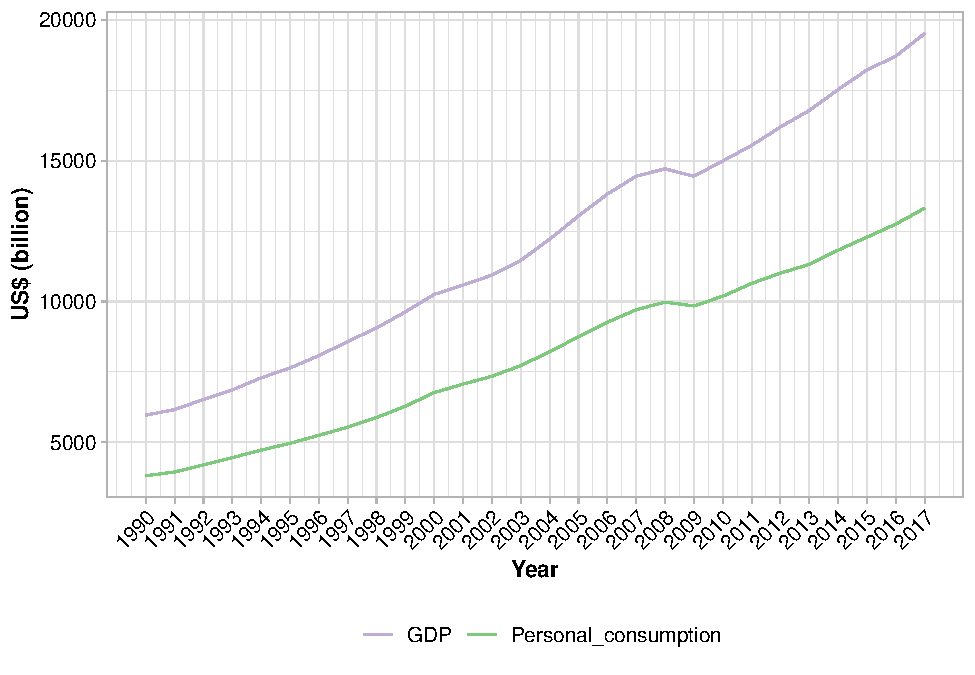
\includegraphics{Project_Code_files/figure-latex/unnamed-chunk-3-1.pdf}
\caption{US Economic Features in 1990-2017}
\end{figure}

\newpage

\subsection{US Electricity
Consumption}\label{us-electricity-consumption}

There were three types of industry sector in the raw dataset. This
project chose to focus on ``Total Electric Industry'', which included
all types of survices in electricity consumption in each sector. There
were four sectors covered in the electricity consumption dataset, which
were illustrated in Table 2. The values of consumption data are in
factor format and separted by commas, so it was necessary to convert
these values to numeric variables first. By visualizing electricity
consumption data in Figure 2, we could observe that all four graphs are
in different consumption scales. Notably, transportation sector had the
lowest electricity consumption among all sectors, and also there was no
data available for transportation sector before 2002. Therefore,
transporation sector would be filtered out in the next step of statistic
analysis.

\begin{Shaded}
\begin{Highlighting}[]
\CommentTok{#Show the structure of the raw dataset}
\KeywordTok{str}\NormalTok{(electric)}
\end{Highlighting}
\end{Shaded}

\begin{verbatim}
## 'data.frame':    5015 obs. of  9 variables:
##  $ Year                    : int  2018 2018 2018 2018 2018 2018 2018 2018 2018 2018 ...
##  $ State                   : Factor w/ 52 levels "AK","AL","AR",..: 1 2 3 4 5 6 7 8 9 10 ...
##  $ Industry.Sector.Category: Factor w/ 3 levels "Energy-Only Providers",..: 3 3 3 3 3 3 3 3 3 3 ...
##  $ Residential             : Factor w/ 3726 levels "0","1,008,481,682",..: 356 2277 1113 2345 3567 1115 669 1332 2906 657 ...
##  $ Commercial              : Factor w/ 3893 levels "0","1","1,000,865,367",..: 1345 1634 609 1878 570 1504 623 3554 2535 3868 ...
##  $ Industrial              : Factor w/ 3883 levels "-229,740","-298,775",..: 161 2341 1147 837 2914 1003 1994 1244 1341 1054 ...
##  $ Transportation          : Factor w/ 663 levels "-26,016","0",..: 2 2 432 592 583 654 102 339 2 614 ...
##  $ Other                   : Factor w/ 1068 levels "-3,968","0","1,016,108",..: NA NA NA NA NA NA NA NA NA NA ...
##  $ Total                   : Factor w/ 3941 levels "0","1,009,966",..: 2723 3808 2576 3463 1539 2856 1665 341 406 1455 ...
\end{verbatim}

\begin{Shaded}
\begin{Highlighting}[]
\CommentTok{#Rename column name for easier use}
\NormalTok{electric <-}\StringTok{ }\NormalTok{electric }\OperatorTok
\StringTok{  }\KeywordTok{rename}\NormalTok{(}\StringTok{'Industry_Sector'}\NormalTok{ =}\StringTok{ }\NormalTok{Industry.Sector.Category, }\StringTok{'elec_residential'}\NormalTok{ =}\StringTok{ }\NormalTok{Residential, }\StringTok{'elec_commercial'}\NormalTok{ =}\StringTok{ }\NormalTok{Commercial, }\StringTok{'elec_industrial'}\NormalTok{ =}\StringTok{ }\NormalTok{Industrial, }\StringTok{'elec_transport'}\NormalTok{ =Transportation)}
\KeywordTok{colnames}\NormalTok{(electric)}
\end{Highlighting}
\end{Shaded}

\begin{verbatim}
## [1] "Year"             "State"            "Industry_Sector" 
## [4] "elec_residential" "elec_commercial"  "elec_industrial" 
## [7] "elec_transport"   "Other"            "Total"
\end{verbatim}

\begin{Shaded}
\begin{Highlighting}[]
\CommentTok{#Reframe dataset to meet project objective}
\NormalTok{elec.select <-}\StringTok{ }\NormalTok{electric }\OperatorTok
\StringTok{  }\KeywordTok{filter}\NormalTok{(State }\OperatorTok{==}\StringTok{ 'US'}\OperatorTok{&}\StringTok{ }\NormalTok{Year}\OperatorTok{>}\DecValTok{1989} \OperatorTok{&}\StringTok{ }\NormalTok{Year }\OperatorTok{<}\StringTok{ }\DecValTok{2018} \OperatorTok{&}\StringTok{ }\NormalTok{Industry_Sector }\OperatorTok{==}\StringTok{ 'Total Electric Industry'}\NormalTok{)}\OperatorTok
\StringTok{  }\KeywordTok{select}\NormalTok{(Year, elec_residential, elec_commercial, elec_industrial, elec_transport) }
\KeywordTok{dim}\NormalTok{(elec.select)}
\end{Highlighting}
\end{Shaded}

\begin{verbatim}
## [1] 28  5
\end{verbatim}

\begin{table}[!h]

\caption{\label{tab:unnamed-chunk-5}First 6 rows of electricity consumptions by sector in US (Mwh)}
\centering
\begin{tabular}{r|l|l|l|l}
\hline
Year & elec\_residential & elec\_commercial & elec\_industrial & elec\_transport\\
\hline
2017 & 1,378,647,742 & 1,352,887,694 & 984,297,945 & 7,522,593\\
\hline
2016 & 1,411,058,153 & 1,367,191,386 & 976,715,181 & 7,496,910\\
\hline
2015 & 1,404,096,499 & 1,360,751,527 & 986,507,732 & 7,636,632\\
\hline
2014 & 1,407,208,311 & 1,352,158,263 & 997,576,138 & 7,757,555\\
\hline
2013 & 1,394,812,129 & 1,337,078,777 & 985,351,874 & 7,625,041\\
\hline
2012 & 1,374,514,708 & 1,327,101,196 & 985,713,854 & 7,320,028\\
\hline
\end{tabular}
\end{table}

\begin{verbatim}
## # A tibble: 1 x 1
##       n
##   <int>
## 1    56
\end{verbatim}

\begin{verbatim}
## 'data.frame':    112 obs. of  3 variables:
##  $ Year                   : int  2017 2016 2015 2014 2013 2012 2011 2010 2009 2008 ...
##  $ Sector                 : chr  "elec_residential" "elec_residential" "elec_residential" "elec_residential" ...
##  $ Electricity_Consumption: num  1.38e+09 1.41e+09 1.40e+09 1.41e+09 1.39e+09 ...
\end{verbatim}

\begin{figure}
\centering
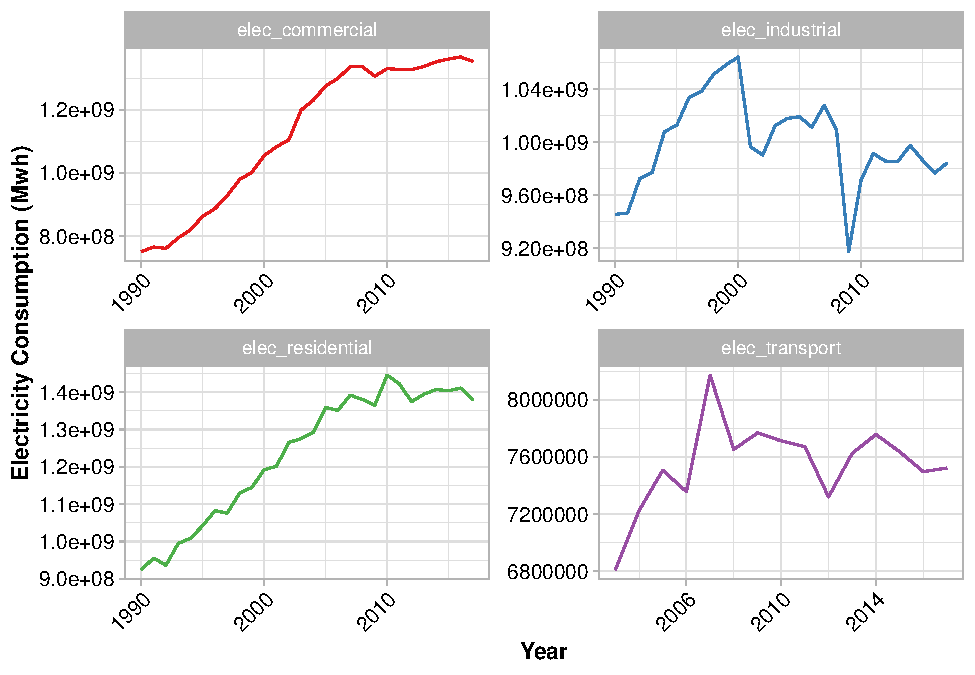
\includegraphics{Project_Code_files/figure-latex/unnamed-chunk-5-1.pdf}
\caption{US Electricty Consumption by Sector in 1990-2017}
\end{figure}

\newpage

\subsection{US GHG Concentration by
Gas}\label{us-ghg-concentration-by-gas}

GHG concentration data refers to the concentration of different GHGs
emitted to the atmosphere. The upper graph in Figure 3 displays the
trends for all GHGs together, from which we can see CO2 was the major
GHG emitted by human beings. To observe the trend of change more
clearly, graphs were created below to show the concentration over years
for each GHG. It was hard to summarize the general trend for all GHG
emissions, so in the next step of analysis, the GHG type comparison
would be first conducted

\begin{Shaded}
\begin{Highlighting}[]
\CommentTok{#Show the structure of the raw data}
\KeywordTok{str}\NormalTok{(GHG.gas)}
\end{Highlighting}
\end{Shaded}

\begin{verbatim}
## 'data.frame':    28 obs. of  6 variables:
##  $ Year             : int  1990 1991 1992 1993 1994 1995 1996 1997 1998 1999 ...
##  $ Carbon.dioxide   : num  5121 5072 5175 5281 5375 ...
##  $ Methane          : num  780 784 783 770 775 ...
##  $ Nitrous.oxide    : num  370 369 372 385 377 ...
##  $ Fluorinated.gases: num  99.7 90.7 95.3 95 98.1 ...
##  $ Total            : num  6371 6316 6425 6532 6625 ...
\end{verbatim}

\begin{Shaded}
\begin{Highlighting}[]
\CommentTok{#Rename column name for easier use}
\KeywordTok{colnames}\NormalTok{(GHG.gas)}
\end{Highlighting}
\end{Shaded}

\begin{verbatim}
## [1] "Year"              "Carbon.dioxide"    "Methane"          
## [4] "Nitrous.oxide"     "Fluorinated.gases" "Total"
\end{verbatim}

\begin{Shaded}
\begin{Highlighting}[]
\NormalTok{GHG.gas <-}\StringTok{ }\NormalTok{GHG.gas }\OperatorTok
\StringTok{  }\KeywordTok{rename}\NormalTok{(}\StringTok{"CO2"}\NormalTok{ =}\StringTok{ }\NormalTok{Carbon.dioxide, }\StringTok{'CH4'}\NormalTok{ =}\StringTok{ }\NormalTok{Methane, }\StringTok{'N2O'}\NormalTok{ =}\StringTok{ }\NormalTok{Nitrous.oxide, }\StringTok{'Fgas'}\NormalTok{ =}\StringTok{ }\NormalTok{Fluorinated.gases)}
\KeywordTok{colnames}\NormalTok{(GHG.gas)}
\end{Highlighting}
\end{Shaded}

\begin{verbatim}
## [1] "Year"  "CO2"   "CH4"   "N2O"   "Fgas"  "Total"
\end{verbatim}

\begin{table}[!h]

\caption{\label{tab:unnamed-chunk-7}First 6 years of GHG emissions by gas type (MMTCO2e)}
\centering
\begin{tabular}{r|r|r|r|r|r}
\hline
Year & CO2 & CH4 & N2O & Fgas & Total\\
\hline
1990 & 5121.179 & 779.8456 & 370.3077 & 99.66786 & 6371.001\\
\hline
1991 & 5071.564 & 784.3849 & 368.9618 & 90.70467 & 6315.615\\
\hline
1992 & 5174.671 & 783.1766 & 371.7864 & 95.30071 & 6424.934\\
\hline
1993 & 5281.387 & 770.3084 & 385.3472 & 95.02735 & 6532.070\\
\hline
1994 & 5375.034 & 775.1607 & 376.5115 & 98.12981 & 6624.836\\
\hline
1995 & 5436.698 & 767.8453 & 388.5028 & 117.02114 & 6710.067\\
\hline
\end{tabular}
\end{table}

\begin{verbatim}
## # A tibble: 1 x 1
##       n
##   <int>
## 1   140
\end{verbatim}

\begin{figure}
\centering
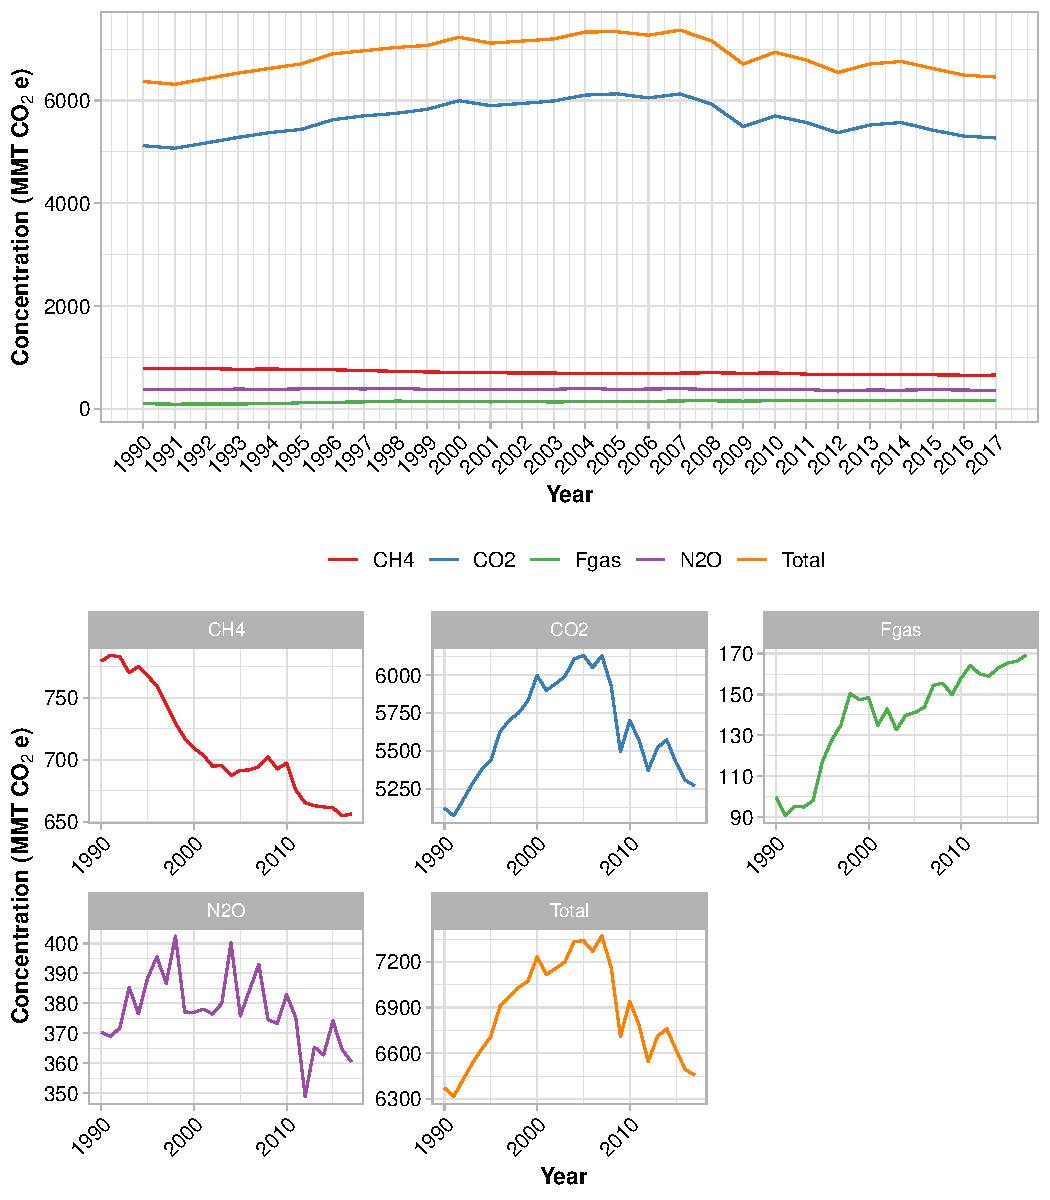
\includegraphics{Project_Code_files/figure-latex/unnamed-chunk-7-1.pdf}
\caption{US GHG Concentration by Gas Type in 1990-2017 (MMTCO2e)}
\end{figure}

\newpage

\subsection{US GHG Emissions by
Sector}\label{us-ghg-emissions-by-sector}

Figure 4 illustrates the GHG emissions over the same period by sector.
The ideology of Figure 4 was same as Figure 3, which internally compared
the emissions by sectors. The total sectoral GHG emission was same as
the sum of GHG concentration by gas type. Among all 6 sectors emitting
GHGs, electricity generation, transporation, and industial sector had
highest emissions. It was inspired to study how sectoral emissions had
contributed to total GHG emissions, and how they were different from
each other.

\begin{Shaded}
\begin{Highlighting}[]
\KeywordTok{str}\NormalTok{(GHG.sector)}
\end{Highlighting}
\end{Shaded}

\begin{verbatim}
## 'data.frame':    28 obs. of  9 variables:
##  $ Year                  : int  1990 1991 1992 1993 1994 1995 1996 1997 1998 1999 ...
##  $ Transportation        : num  1527 1481 1541 1578 1632 ...
##  $ Electricity.generation: num  1876 1872 1887 1962 1987 ...
##  $ Industry              : num  1629 1601 1632 1605 1630 ...
##  $ Agriculture           : num  535 535 539 552 544 ...
##  $ Commercial            : num  427 434 429 425 427 ...
##  $ Residential           : num  345 354 361 372 363 ...
##  $ U.S..territories      : num  33.3 39.1 37.3 39.1 41.5 ...
##  $ Total                 : num  6371 6316 6425 6532 6625 ...
\end{verbatim}

\begin{Shaded}
\begin{Highlighting}[]
\CommentTok{#Rename column name for easier use}
\KeywordTok{colnames}\NormalTok{(GHG.sector)}
\end{Highlighting}
\end{Shaded}

\begin{verbatim}
## [1] "Year"                   "Transportation"        
## [3] "Electricity.generation" "Industry"              
## [5] "Agriculture"            "Commercial"            
## [7] "Residential"            "U.S..territories"      
## [9] "Total"
\end{verbatim}

\begin{Shaded}
\begin{Highlighting}[]
\NormalTok{GHG.sector <-}\StringTok{ }\NormalTok{GHG.sector }\OperatorTok
\StringTok{  }\KeywordTok{rename}\NormalTok{(}\StringTok{'Electricity_generation'}\NormalTok{ =}\StringTok{ }\NormalTok{Electricity.generation)}
\KeywordTok{colnames}\NormalTok{(GHG.sector)}
\end{Highlighting}
\end{Shaded}

\begin{verbatim}
## [1] "Year"                   "Transportation"        
## [3] "Electricity_generation" "Industry"              
## [5] "Agriculture"            "Commercial"            
## [7] "Residential"            "U.S..territories"      
## [9] "Total"
\end{verbatim}

\begin{Shaded}
\begin{Highlighting}[]
\CommentTok{#Reframe dataset to meet project objective}
\NormalTok{GHG.sector.select <-}\StringTok{ }\NormalTok{GHG.sector }\OperatorTok
\StringTok{  }\KeywordTok{select}\NormalTok{(Year, Transportation, Electricity_generation, Industry, Agriculture, Commercial,Residential)}
\KeywordTok{dim}\NormalTok{(GHG.sector.select)}
\end{Highlighting}
\end{Shaded}

\begin{verbatim}
## [1] 28  7
\end{verbatim}

\begin{table}[!h]

\caption{\label{tab:unnamed-chunk-9}First 6 years of GHG emissions by sector (MMTCO2e)}
\centering
\begin{tabular}{r|r|r|r|r|r|r}
\hline
Year & Transportation & Electricity\_generation & Industry & Agriculture & Commercial & Residential\\
\hline
1990 & 1527.077 & 1875.537 & 1628.556 & 534.8599 & 426.9285 & 344.7218\\
\hline
1991 & 1480.932 & 1871.568 & 1601.088 & 534.6403 & 433.9764 & 354.2868\\
\hline
1992 & 1540.536 & 1886.539 & 1631.550 & 538.7436 & 429.4007 & 360.8492\\
\hline
1993 & 1577.523 & 1962.302 & 1604.889 & 551.5106 & 424.5561 & 372.2031\\
\hline
1994 & 1632.154 & 1987.103 & 1629.785 & 543.9804 & 427.1918 & 363.1420\\
\hline
1995 & 1667.330 & 2003.827 & 1647.961 & 556.7418 & 426.3748 & 367.4087\\
\hline
\end{tabular}
\end{table}

\begin{verbatim}
## # A tibble: 1 x 1
##       n
##   <int>
## 1   168
\end{verbatim}

\begin{figure}
\centering
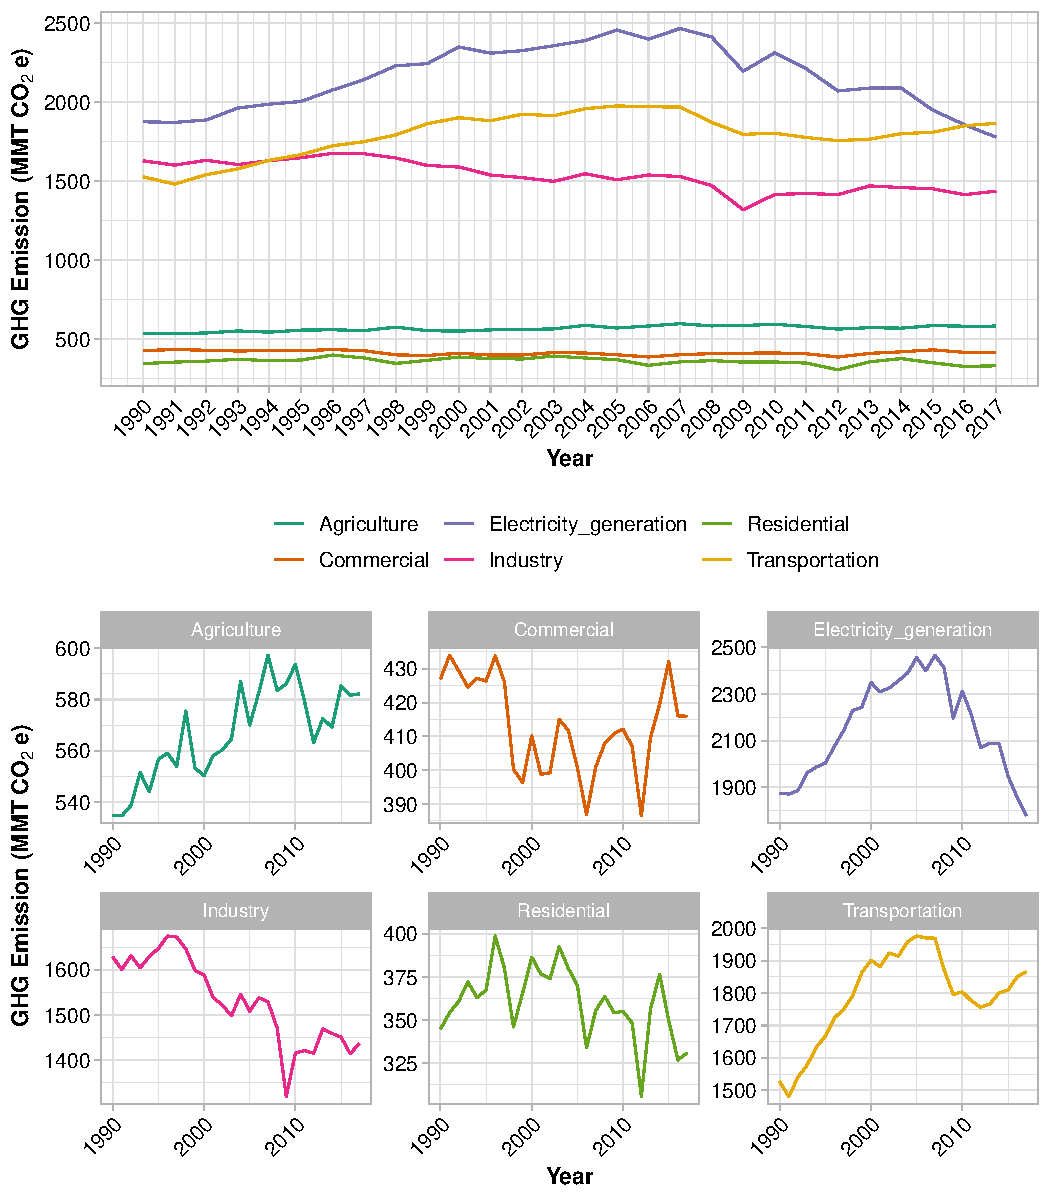
\includegraphics{Project_Code_files/figure-latex/unnamed-chunk-10-1.pdf}
\caption{US GHG Emissions by Sector in 1990-2017 (MMTCO2e)}
\end{figure}

\newpage

\subsection{US Mean Annual
Temperature}\label{us-mean-annual-temperature}

Mean annual temperature and temperature anomalies over 1990-2017 were
visualized in Figure 5. Temperature anomaly refers to the difference
between annual mean temperature and overall averaage temperature for
that period. Therefore, the overall average temperature were also
calculated and mutated as a new column in the table. Since overall
average temperature is constant, temperature anomalies are in the same
changing trends as annual mean temperature. As referene values,
temperature anomalies can better and more easily demonstrate increasing
and decreasing trends by positive and negative symbols. Therefore,
temperature anomaly would be used in the future analyses.

\begin{Shaded}
\begin{Highlighting}[]
\KeywordTok{str}\NormalTok{(temp)}
\end{Highlighting}
\end{Shaded}

\begin{verbatim}
## 'data.frame':    28 obs. of  3 variables:
##  $ Date   : int  199012 199112 199212 199312 199412 199512 199612 199712 199812 199912 ...
##  $ Value  : num  53.5 53.2 52.6 51.3 52.9 ...
##  $ Anomaly: num  0.25 -0.1 -0.66 -2 -0.39 -0.61 -1.38 -1.06 0.97 0.62 ...
\end{verbatim}

\begin{Shaded}
\begin{Highlighting}[]
\CommentTok{#Convert year characters to date format}
\KeywordTok{colnames}\NormalTok{(temp)}
\end{Highlighting}
\end{Shaded}

\begin{verbatim}
## [1] "Date"    "Value"   "Anomaly"
\end{verbatim}

\begin{Shaded}
\begin{Highlighting}[]
\NormalTok{temp <-}\StringTok{ }\KeywordTok{mutate}\NormalTok{(temp, }\DataTypeTok{Year =} \KeywordTok{year}\NormalTok{(}\KeywordTok{as.Date}\NormalTok{(}\KeywordTok{as.yearmon}\NormalTok{(}\KeywordTok{as.character}\NormalTok{(temp}\OperatorTok{$}\NormalTok{Date), }\DataTypeTok{format =} \StringTok{"%Y%m"}\NormalTok{))))}
\KeywordTok{str}\NormalTok{(temp)}
\end{Highlighting}
\end{Shaded}

\begin{verbatim}
## 'data.frame':    28 obs. of  4 variables:
##  $ Date   : int  199012 199112 199212 199312 199412 199512 199612 199712 199812 199912 ...
##  $ Value  : num  53.5 53.2 52.6 51.3 52.9 ...
##  $ Anomaly: num  0.25 -0.1 -0.66 -2 -0.39 -0.61 -1.38 -1.06 0.97 0.62 ...
##  $ Year   : num  1990 1991 1992 1993 1994 ...
\end{verbatim}

\begin{Shaded}
\begin{Highlighting}[]
\CommentTok{#Reframe dataset to meet project objective}
\NormalTok{temp.select <-}\StringTok{ }\NormalTok{temp }\OperatorTok
\StringTok{  }\KeywordTok{select}\NormalTok{(Year, Value, Anomaly) }\OperatorTok
\StringTok{  }\KeywordTok{mutate}\NormalTok{(}\DataTypeTok{Mean_all_temp =}  \KeywordTok{mean}\NormalTok{(Value))}
\KeywordTok{dim}\NormalTok{(temp.select)}
\end{Highlighting}
\end{Shaded}

\begin{verbatim}
## [1] 28  4
\end{verbatim}

\begin{Shaded}
\begin{Highlighting}[]
\KeywordTok{str}\NormalTok{(temp.select)}
\end{Highlighting}
\end{Shaded}

\begin{verbatim}
## 'data.frame':    28 obs. of  4 variables:
##  $ Year         : num  1990 1991 1992 1993 1994 ...
##  $ Value        : num  53.5 53.2 52.6 51.3 52.9 ...
##  $ Anomaly      : num  0.25 -0.1 -0.66 -2 -0.39 -0.61 -1.38 -1.06 0.97 0.62 ...
##  $ Mean_all_temp: num  53.3 53.3 53.3 53.3 53.3 ...
\end{verbatim}

\begin{table}[!h]

\caption{\label{tab:unnamed-chunk-12}First 6 years of US temperature data in 1990-2017 (F)}
\centering
\begin{tabular}{r|r|r|r}
\hline
Year & Value & Anomaly & Mean\_all\_temp\\
\hline
1990 & 53.51 & 0.25 & 53.25964\\
\hline
1991 & 53.16 & -0.10 & 53.25964\\
\hline
1992 & 52.60 & -0.66 & 53.25964\\
\hline
1993 & 51.26 & -2.00 & 53.25964\\
\hline
1994 & 52.87 & -0.39 & 53.25964\\
\hline
1995 & 52.65 & -0.61 & 53.25964\\
\hline
\end{tabular}
\end{table}

\begin{figure}
\centering
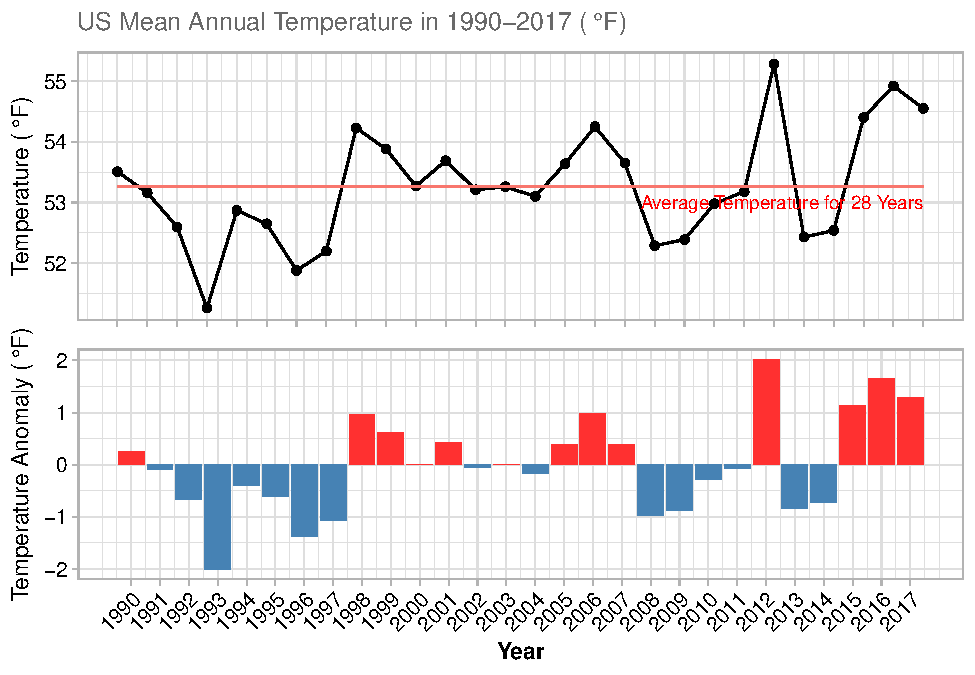
\includegraphics{Project_Code_files/figure-latex/unnamed-chunk-13-1.pdf}
\caption{US Mean Annual Temperature Anomaly in 1990-2017 (F)}
\end{figure}

\newpage

\subsection{US Population}\label{us-population}

Population data retrieved from World Bank is at global scale covering 60
years since 1960. Therefore, both geograhic and temporal selection of
the dataset have to be reframed. The sample of the wrangled dateset was
shown as Table 6.

\begin{Shaded}
\begin{Highlighting}[]
\KeywordTok{str}\NormalTok{(ppl)}
\end{Highlighting}
\end{Shaded}

\begin{verbatim}
## 'data.frame':    60 obs. of  265 variables:
##  $ Year                                                : int  1960 1961 1962 1963 1964 1965 1966 1967 1968 1969 ...
##  $ Aruba                                               : int  54211 55438 56225 56695 57032 57360 57715 58055 58386 58726 ...
##  $ Afghanistan                                         : int  8996973 9169410 9351441 9543205 9744781 9956320 10174836 10399926 10637063 10893776 ...
##  $ Angola                                              : int  5454933 5531472 5608539 5679458 5735044 5770570 5781214 5774243 5771652 5803254 ...
##  $ Albania                                             : int  1608800 1659800 1711319 1762621 1814135 1864791 1914573 1965598 2022272 2081695 ...
##  $ Andorra                                             : int  13411 14375 15370 16412 17469 18549 19647 20758 21890 23058 ...
##  $ Arab.World                                          : int  92197753 94724510 97334442 100034179 102832760 105736431 108758610 111899364 115136178 118437195 ...
##  $ United.Arab.Emirates                                : int  92418 100796 112118 125130 138039 149857 159976 169771 182627 203106 ...
##  $ Argentina                                           : int  20481779 20817266 21153052 21488912 21824425 22159650 22494035 22828869 23168267 23517611 ...
##  $ Armenia                                             : int  1874121 1941492 2009526 2077578 2145001 2211319 2276034 2339127 2401143 2462928 ...
##  $ American.Samoa                                      : int  20123 20602 21253 22034 22854 23672 24462 25248 25989 26703 ...
##  $ Antigua.and.Barbuda                                 : int  54131 55001 55841 56702 57641 58698 59915 61241 62521 63550 ...
##  $ Australia                                           : int  10276477 10483000 10742000 10950000 11167000 11388000 11651000 11799000 12009000 12263000 ...
##  $ Austria                                             : int  7047539 7086299 7129864 7175811 7223801 7270889 7322066 7376998 7415403 7441055 ...
##  $ Azerbaijan                                          : int  3895397 4030322 4171426 4315127 4456687 4592609 4721523 4843868 4960232 5071927 ...
##  $ Burundi                                             : int  2797932 2852438 2907321 2964427 3026290 3094379 3170490 3253218 3336927 3413904 ...
##  $ Belgium                                             : int  9153489 9183948 9220578 9289770 9378113 9463667 9527807 9580991 9618756 9646032 ...
##  $ Benin                                               : int  2431622 2465867 2502896 2542859 2585965 2632356 2682159 2735307 2791590 2850661 ...
##  $ Burkina.Faso                                        : int  4829288 4894580 4960326 5027821 5098890 5174870 5256363 5343019 5434041 5528174 ...
##  $ Bangladesh                                          : int  48013504 49362843 50752157 52202007 53741716 55385112 57157654 59034249 60918454 62679765 ...
##  $ Bulgaria                                            : int  7867374 7943118 8012946 8078145 8144340 8204168 8258057 8310226 8369603 8434172 ...
##  $ Bahrain                                             : int  162427 167894 173144 178140 182887 187431 191780 196063 200653 206043 ...
##  $ Bahamas..The                                        : int  109534 115121 121091 127339 133709 140059 146382 152620 158648 164268 ...
##  $ Bosnia.and.Herzegovina                              : int  3225668 3288603 3353226 3417574 3478997 3535643 3586636 3632672 3675454 3717468 ...
##  $ Belarus                                             : int  8198000 8271216 8351928 8437232 8524224 8610000 8696496 8785648 8874552 8960304 ...
##  $ Belize                                              : int  92064 94703 97384 100164 103069 106119 109347 112692 116061 119261 ...
##  $ Bermuda                                             : int  44400 45500 46600 47700 48900 50100 51000 52000 53000 54000 ...
##  $ Bolivia                                             : int  3656955 3728964 3802990 3879192 3957757 4038872 4122517 4208676 4297517 4389246 ...
##  $ Brazil                                              : int  72179226 74311343 76514328 78772657 81064571 83373530 85696505 88035814 90387079 92746614 ...
##  $ Barbados                                            : int  230980 231718 232633 233630 234586 235413 236088 236659 237241 237955 ...
##  $ Brunei.Darussalam                                   : int  81702 85562 89481 93540 97812 102386 107274 112448 117898 123600 ...
##  $ Bhutan                                              : int  223288 228851 234554 240523 246964 253994 261668 269947 278734 287891 ...
##  $ Botswana                                            : int  502745 512685 523778 535685 547873 559994 571964 584092 596947 611300 ...
##  $ Central.African.Republic                            : int  1501668 1526066 1551910 1579370 1608616 1639706 1673019 1708302 1744194 1778861 ...
##  $ Canada                                              : int  17909009 18271000 18614000 18964000 19325000 19678000 20048000 20412000 20744000 21028000 ...
##  $ Central.Europe.and.the.Baltics                      : int  91401764 92232738 93009498 93840016 94715795 95440988 96146336 97043270 97884022 98606630 ...
##  $ Switzerland                                         : int  5327827 5434294 5573815 5694247 5789228 5856472 5918002 5991785 6067714 6136387 ...
##  $ Channel.Islands                                     : int  109420 110399 111457 112595 113773 114995 116227 117474 118726 119972 ...
##  $ Chile                                               : int  8132990 8303811 8476897 8650387 8821858 8989621 9152844 9312095 9468845 9625312 ...
##  $ China                                               : int  667070000 660330000 665770000 682335000 698355000 715185000 735400000 754550000 774510000 796025000 ...
##  $ Cote.d.Ivoire                                       : int  3503553 3631553 3770766 3918628 4071411 4226844 4383728 4544164 4713135 4897472 ...
##  $ Cameroon                                            : int  5176918 5285017 5398729 5518104 5643036 5773543 5909882 6052420 6201413 6357092 ...
##  $ Congo..Dem..Rep.                                    : int  15248251 15637699 16041190 16461830 16903831 17369883 17862049 18378625 18913878 19459816 ...
##  $ Congo..Rep.                                         : int  1018253 1043116 1069238 1096638 1125352 1155392 1186785 1219541 1253760 1289522 ...
##  $ Colombia                                            : int  16057724 16567811 17092918 17629979 18175185 18725245 19279740 19837510 20393699 20942456 ...
##  $ Comoros                                             : int  191121 194139 197198 200372 203753 207424 211478 215897 220575 225325 ...
##  $ Cabo.Verde                                          : int  201765 205327 210142 216096 222948 230418 238655 247527 256176 263453 ...
##  $ Costa.Rica                                          : int  1330782 1381183 1433335 1486553 1539941 1592841 1645083 1696732 1747694 1797893 ...
##  $ Caribbean.small.states                              : int  4194710 4274060 4353628 4432217 4508198 4580374 4648367 4712526 4773902 4833842 ...
##  $ Cuba                                                : int  7141250 7291200 7453540 7623294 7793262 7958169 8115487 8266380 8413552 8561384 ...
##  $ Curacao                                             : int  124826 126125 128414 130860 133148 135266 136682 138140 140298 142581 ...
##  $ Cayman.Islands                                      : int  7865 8026 8146 8227 8298 8369 8441 8522 8631 8827 ...
##  $ Cyprus                                              : int  572930 576395 577691 577913 578625 580966 585309 591308 598495 606116 ...
##  $ Czech.Republic                                      : int  9602006 9586651 9624660 9670685 9727804 9779358 9821040 9852899 9876346 9896580 ...
##  $ Germany                                             : int  72814900 73377632 74025784 74714353 75318337 75963695 76600311 76951336 77294314 77909682 ...
##  $ Djibouti                                            : int  83636 88498 94204 100628 107583 114963 122866 131397 140462 149887 ...
##  $ Dominica                                            : int  60011 61032 61982 62918 63926 65038 66311 67686 69040 70213 ...
##  $ Denmark                                             : int  4579603 4611687 4647727 4684483 4722072 4759012 4797381 4835354 4864883 4891860 ...
##  $ Dominican.Republic                                  : int  3294224 3406280 3521018 3638109 3757132 3877765 3999796 4123092 4247558 4373124 ...
##  $ Algeria                                             : int  11057863 11336339 11619828 11912803 12221675 12550885 12902627 13275026 13663583 14061722 ...
##  $ East.Asia...Pacific..excluding.high.income.         : int  894880101 894484115 906418827 929639988 952499842 976366448 1003805626 1030347262 1057855221 1087061065 ...
##  $ Early.demographic.dividend                          : num  9.80e+08 1.00e+09 1.03e+09 1.05e+09 1.08e+09 ...
##  $ East.Asia...Pacific                                 : num  1.04e+09 1.04e+09 1.06e+09 1.08e+09 1.11e+09 ...
##  $ Europe...Central.Asia..excluding.high.income.       : int  275147578 279443876 283762877 288099625 292424434 296682673 300278116 303940876 307516657 311023409 ...
##  $ Europe...Central.Asia                               : int  667253650 674962981 682921730 690946639 698901133 706626086 713395321 719979928 726307440 732494115 ...
##  $ Ecuador                                             : int  4543666 4674172 4809201 4948986 5093854 5243977 5399422 5560012 5725459 5895367 ...
##  $ Egypt..Arab.Rep.                                    : int  26632894 27366237 28112256 28871383 29644875 30433022 31237600 32056510 32881848 33703139 ...
##  $ Euro.area                                           : int  265203934 267621101 270110056 272655378 275163387 277650957 279969040 281974883 283866409 285778637 ...
##  $ Eritrea                                             : int  1007590 1033328 1060486 1088854 1118159 1148189 1178875 1210302 1242635 1276123 ...
##  $ Spain                                               : int  30455000 30739250 31023366 31296651 31609195 31954292 32283194 32682947 33113134 33441054 ...
##  $ Estonia                                             : int  1211537 1225077 1241623 1258857 1277086 1294566 1308597 1318946 1331214 1345249 ...
##  $ Ethiopia                                            : int  22151278 22671191 23221389 23798430 24397022 25013626 25641044 26280132 26944390 27652709 ...
##  $ European.Union                                      : int  356906076 359998418 363200473 366516491 369850244 373032732 376039119 378917977 381605443 384216975 ...
##  $ Fragile.and.conflict.affected.situations            : int  174658134 178611702 182724039 186993460 191428676 196036841 200829540 205811110 210968809 216287242 ...
##  $ Finland                                             : int  4429634 4461005 4491443 4523309 4548543 4563732 4580869 4605744 4626469 4623785 ...
##  $ Fiji                                                : int  393481 407249 421665 436293 450542 463968 476404 487981 498940 509704 ...
##  $ France                                              : int  46621669 47240543 47904877 48582611 49230595 49818028 50330262 50775794 51175508 51561836 ...
##  $ Faroe.Islands                                       : int  34615 35076 35524 35969 36406 36847 37278 37705 38124 38570 ...
##  $ Micronesia..Fed..Sts.                               : int  44514 45932 47367 48855 50468 52227 54192 56307 58388 60145 ...
##  $ Gabon                                               : int  500928 505799 511287 517580 524895 533361 543112 554059 565766 577646 ...
##  $ United.Kingdom                                      : int  52400000 52800000 53250000 53650000 54000000 54348050 54648500 54943600 55211700 55441750 ...
##  $ Georgia                                             : int  3645600 3703600 3760300 3816100 3870300 3921600 3966700 4005800 4042300 4080300 ...
##  $ Ghana                                               : int  6635230 6848295 7071971 7300116 7524472 7739473 7941412 8132803 8321770 8520015 ...
##  $ Gibraltar                                           : int  23420 23813 24313 24889 25479 26073 26633 27173 27685 28166 ...
##  $ Guinea                                              : int  3494162 3552065 3611429 3672556 3735916 3801705 3870203 3941053 4013055 4084600 ...
##  $ Gambia..The                                         : int  365047 372445 379894 387641 396011 405259 415478 426629 438603 451228 ...
##  $ Guinea.Bissau                                       : int  616136 622761 628883 635011 641812 649790 658994 669237 680432 692407 ...
##  $ Equatorial.Guinea                                   : int  255333 258791 262219 266000 270618 276300 283506 291790 299413 304000 ...
##  $ Greece                                              : int  8331725 8398050 8448233 8479625 8510429 8550333 8613651 8684088 8740765 8772764 ...
##  $ Grenada                                             : int  89932 91327 92484 93413 94123 94636 94934 95020 94927 94728 ...
##  $ Greenland                                           : int  32500 33700 35000 36400 37600 39200 40500 41900 43400 44900 ...
##  $ Guatemala                                           : int  4210747 4336143 4464249 4595510 4730540 4869716 5013153 5160609 5311615 5465512 ...
##  $ Guam                                                : int  66742 68072 69604 71286 73051 74830 76607 78404 80217 82040 ...
##  $ Guyana                                              : int  571819 589274 606285 622575 637845 651868 664521 675871 686146 695745 ...
##  $ High.income                                         : int  760193906 771546780 781558432 791500756 801349486 810831993 819708674 827927262 835367980 844677617 ...
##  $ Hong.Kong.SAR..China                                : int  3075605 3168100 3305200 3420900 3504600 3597900 3629900 3722800 3802700 3863900 ...
##  $ Honduras                                            : int  2038632 2096409 2155647 2216704 2280048 2346015 2414803 2486415 2560727 2637513 ...
##  $ Heavily.indebted.poor.countries..HIPC.              : int  161734357 165573152 169567094 173722855 178048171 182548785 187227582 192084649 197119436 202329943 ...
##  $ Croatia                                             : int  4140181 4167292 4196712 4225675 4252876 4280923 4310701 4338683 4365628 4391490 ...
##   [list output truncated]
\end{verbatim}

\begin{Shaded}
\begin{Highlighting}[]
\CommentTok{#Reframe dataset to meet project objective}
\NormalTok{ppl.select <-}\StringTok{ }\NormalTok{ppl }\OperatorTok
\StringTok{  }\KeywordTok{select}\NormalTok{(Year, United.States) }\OperatorTok
\StringTok{  }\KeywordTok{filter}\NormalTok{(Year }\OperatorTok{>}\DecValTok{1989} \OperatorTok{&}\StringTok{ }\NormalTok{Year }\OperatorTok{<}\StringTok{ }\DecValTok{2018}\NormalTok{)}
\KeywordTok{dim}\NormalTok{(ppl.select)}
\end{Highlighting}
\end{Shaded}

\begin{verbatim}
## [1] 28  2
\end{verbatim}

\begin{Shaded}
\begin{Highlighting}[]
\CommentTok{#Rename column name for easier use}
\KeywordTok{colnames}\NormalTok{(ppl.select)}
\end{Highlighting}
\end{Shaded}

\begin{verbatim}
## [1] "Year"          "United.States"
\end{verbatim}

\begin{Shaded}
\begin{Highlighting}[]
\NormalTok{ppl.select <-}\StringTok{ }\NormalTok{ppl.select }\OperatorTok
\StringTok{  }\KeywordTok{rename}\NormalTok{(}\StringTok{'US_pop'}\NormalTok{ =}\StringTok{ }\NormalTok{United.States)}
\KeywordTok{colnames}\NormalTok{(ppl.select)}
\end{Highlighting}
\end{Shaded}

\begin{verbatim}
## [1] "Year"   "US_pop"
\end{verbatim}

\begin{table}[!h]

\caption{\label{tab:unnamed-chunk-15}First 6 years of US population in 1990-2017}
\centering
\begin{tabular}{r|r}
\hline
Year & US\_pop\\
\hline
1990 & 249623000\\
\hline
1991 & 252981000\\
\hline
1992 & 256514000\\
\hline
1993 & 259919000\\
\hline
1994 & 263126000\\
\hline
1995 & 266278000\\
\hline
\end{tabular}
\end{table}

\begin{Shaded}
\begin{Highlighting}[]
\CommentTok{#Save all processed code to the Processed folder}
\KeywordTok{write.csv}\NormalTok{(GDP.select, }\DataTypeTok{row.names =} \OtherTok{FALSE}\NormalTok{, }\DataTypeTok{file =} \StringTok{'./Processed Data/BEA_GDP_processed.csv'}\NormalTok{)}
\KeywordTok{write.csv}\NormalTok{(elec.select, }\DataTypeTok{row.names =} \OtherTok{FALSE}\NormalTok{, }\DataTypeTok{file =} \StringTok{'./Processed Data/EIA_electricity-consumption_sector_processed.csv'}\NormalTok{)}
\KeywordTok{write.csv}\NormalTok{(GHG.gas, }\DataTypeTok{row.names =} \OtherTok{FALSE}\NormalTok{, }\DataTypeTok{file =} \StringTok{'./Processed Data/EPA_GHG_Gas_processed.csv'}\NormalTok{)}
\KeywordTok{write.csv}\NormalTok{(GHG.sector.select, }\DataTypeTok{row.names =} \OtherTok{FALSE}\NormalTok{, }\DataTypeTok{file =} \StringTok{'./Processed Data/EPA_GHG_Sector_processed.csv'}\NormalTok{)}
\KeywordTok{write.csv}\NormalTok{(temp.select, }\DataTypeTok{row.names =} \OtherTok{FALSE}\NormalTok{, }\DataTypeTok{file =} \StringTok{'./Processed Data/NOAA_temp_processed.csv'}\NormalTok{)}
\KeywordTok{write.csv}\NormalTok{(ppl.select, }\DataTypeTok{row.names =} \OtherTok{FALSE}\NormalTok{, }\DataTypeTok{file =} \StringTok{'./Processed Data/WB_pop_processed.csv'}\NormalTok{)}
\end{Highlighting}
\end{Shaded}

\begin{Shaded}
\begin{Highlighting}[]
\CommentTok{#Reload new datasets}
\NormalTok{newGDP <-}\StringTok{ }\KeywordTok{read.csv}\NormalTok{(}\StringTok{'./Processed Data/BEA_GDP_processed.csv'}\NormalTok{, }\KeywordTok{head}\NormalTok{(T))}
\NormalTok{newelectricity <-}\StringTok{ }\KeywordTok{read.csv}\NormalTok{(}\StringTok{'./Processed Data/EIA_electricity-consumption_sector_processed.csv'}\NormalTok{, }\KeywordTok{head}\NormalTok{(T))}
\NormalTok{newGHGgas <-}\StringTok{ }\KeywordTok{read.csv}\NormalTok{(}\StringTok{'./Processed Data/EPA_GHG_Gas_processed.csv'}\NormalTok{, }\KeywordTok{head}\NormalTok{(T))}
\NormalTok{newGHGsector <-}\StringTok{ }\KeywordTok{read.csv}\NormalTok{(}\StringTok{'./Processed Data/EPA_GHG_Sector_processed.csv'}\NormalTok{, }\KeywordTok{head}\NormalTok{(T))}
\NormalTok{newtemp <-}\StringTok{ }\KeywordTok{read.csv}\NormalTok{(}\StringTok{'./Processed Data/NOAA_temp_processed.csv'}\NormalTok{, }\KeywordTok{head}\NormalTok{(T))}
\NormalTok{newpop <-}\StringTok{ }\KeywordTok{read.csv}\NormalTok{(}\StringTok{'./Processed Data/WB_pop_processed.csv'}\NormalTok{, }\KeywordTok{head}\NormalTok{(T))}

\NormalTok{allGHG <-}\StringTok{ }\KeywordTok{full_join}\NormalTok{(newGHGgas,newGHGsector, }\DataTypeTok{by =} \StringTok{'Year'}\NormalTok{)}
\NormalTok{GHG_contribute <-}\StringTok{ }\KeywordTok{full_join}\NormalTok{(newelectricity, newpop, }\DataTypeTok{by =} \StringTok{'Year'}\NormalTok{)}
\NormalTok{GHG_impact <-}\StringTok{ }\KeywordTok{full_join}\NormalTok{(newGDP, newtemp, }\DataTypeTok{by =} \StringTok{'Year'}\NormalTok{)}
\end{Highlighting}
\end{Shaded}

\newpage

\section{Analysis}\label{analysis}

\emph{Figures in this sections are disordered - the float package was
not compatible to my system. Texts in this section will specify which
figures are referring to in certain analyses.}

\subsection{Question 1: What factors have contributed to GHG emissions
in these 28
years?}\label{question-1-what-factors-have-contributed-to-ghg-emissions-in-these-28-years}

\subsubsection{Were emissions of different GHGs related to each
other?}\label{were-emissions-of-different-ghgs-related-to-each-other}

As discussed in Chapter 3, there was no general trend for the
concentration of all GHGs. Therefore, before delving into external
impacts on GHG concentrations, how different types of GHGs were varied
from each other were first studied.

The distribution of all GHG data were assessed with shapiro.test. Most
p-values were greater than 0.05, which implied that the distribution of
these data were not significantly different from normal distribution.
Therefore, these data were normally distributed. Other data, namely CH4
and Fgas, obtained a p-value less than 0.05 (even transforming these two
variables by taking the log and square root), which indicated they were
not normally distributed. However, from the normal Q-Q plot, the
scatters lied close to the line and symmetry across the qq normal line,
so these two data could still be seen as normally distributed. All GHG
emissions by sector obtained p-values greater than 0.05 from the
shapiro.test, so they were normally distributed. Parametric tests would
be used for all GHG dataset.

Multiple Linear Regression was conducted between CO2 and other GHGs to
see if there could be any relationships between CO2 and other GHGs, as
there are always multiple GHGs emitted together by one source. The
result illustarted that at least one of GHGs was significantly related
to the CO2 emission (linear regression; R2=0.5562, dF = 24, p =
0.0001805). Specifically, changes in N2O emissions were significantly
related to changes in CO2 emissions, while changes in CH4 and Fgas were
not significantly related to CO2 emissions.

To step further, a correlation plot was created to reveal the possible
relationships, as well as covariance among explanatory variables, as
shown in Figure 6, in which blue indiates positively correlated and red
indicate negatively correlated. The smaller ellipse indicates a higher
correlationship between two variables, and the dark color implies a
higher correlation cofficient. Therefore, both N2O and Fgas had positive
correlationships with CO2, but N2O was more correlated and had a higher
correlation coeffeicnt; on the other hand, CH4 had a negative
correlationship with CO2 and such correlation was not significant as the
ellipse was large. However, it was interesting to see CH4 and Fgas had a
strong negative correlationship. Another format to observe the
correlationship with CO2 concentration was shown in Figure 7.

Based on this reuslt, Akaike's Information Criterion (AIC) were computed
to improve the model to best predict impacts on CO2 emission, from which
only N2O and CH4 were remained in the improved model (Step: AIC=306.73).
The improved model implied that both CH4 and N2O emissions were
significantly related to CO2 emissions (linear regression; R2=0.5461, dF
= 25, p \textless{} 0.0001).

\begin{figure}
\centering
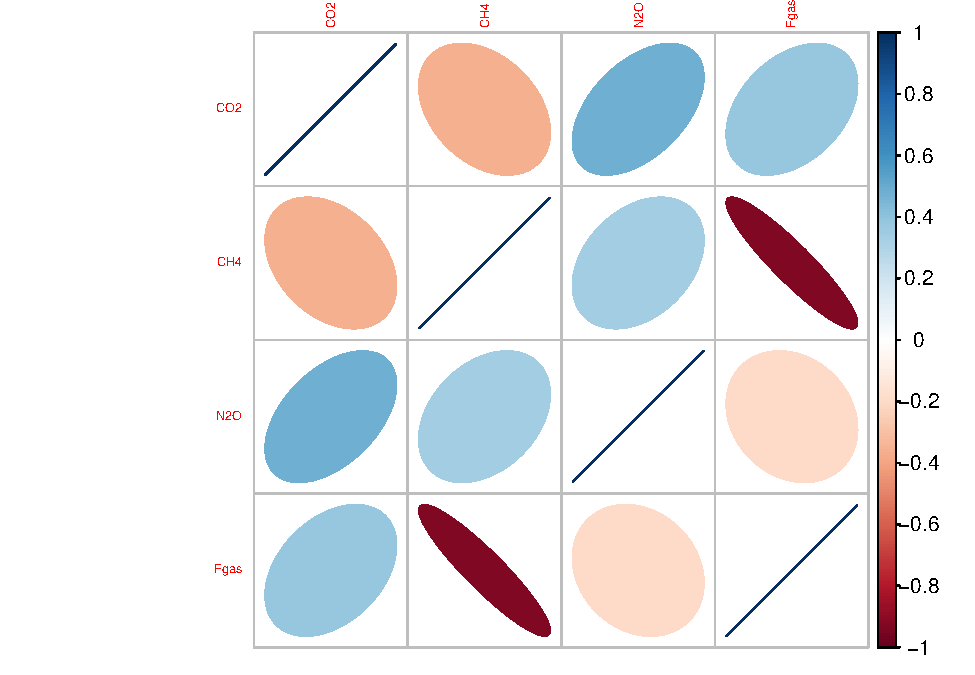
\includegraphics{Project_Code_files/figure-latex/unnamed-chunk-20-1.pdf}
\caption{Correlation Plot of US GHG Concentration by Gas}
\end{figure}

\begin{figure}
\centering
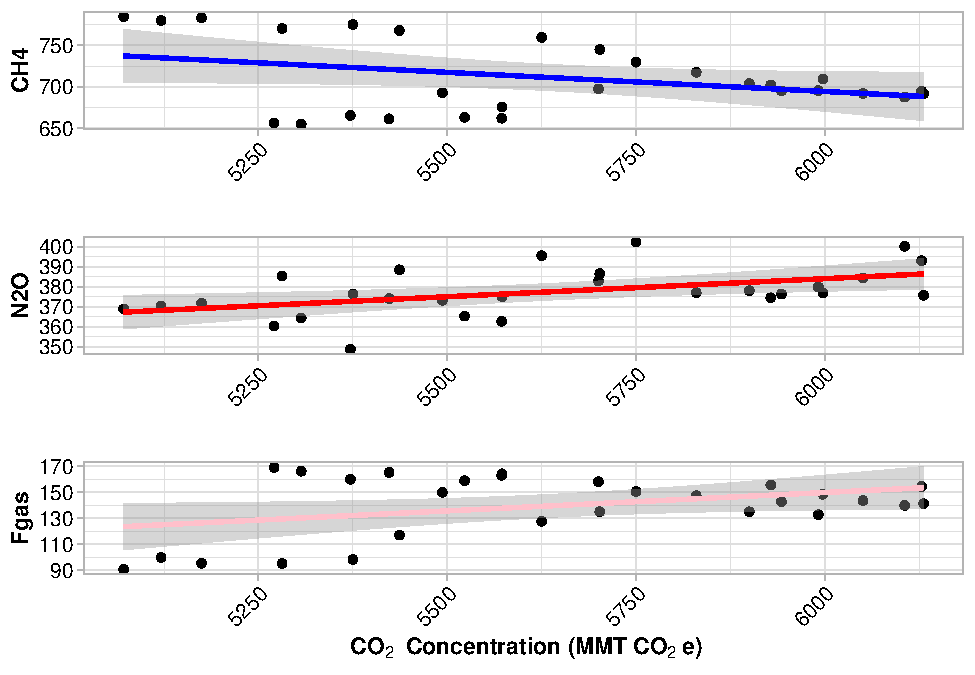
\includegraphics{Project_Code_files/figure-latex/unnamed-chunk-21-1.pdf}
\caption{Correlationships between CO2 and other GHGs}
\end{figure}

\newpage

Similarly, multiple Linear Regression was also conducted among sectoral
GHG emissions to see which sector was significant to electricity
generation sector, which had the highest GHG emissions.

The result illustarted that multiple sectors had significant
relationships with electricity generation sector (linear regression;
R2=0.8566, dF = 22, p \textless{} 0.0001). Specifically, emission
changes in agriculture, commercial, and residential sectors were
significantly related to emission changes in electricity generation
sector, while changes in transporation and industry sectors were not
significantly related to electricity generation emissions. This result
was also proved by AIC test that best model would be three significant
explanatory variables.

The correlation plot in Figure 8 shows some interesting results of
covariances among expanatory variables. Transporation sector was more
positively correlated to electricity generation than agriculture and
residential sectors. Industry sector had litte correlation with
electricity generation while commercial was negatively correlated.

\begin{figure}
\centering
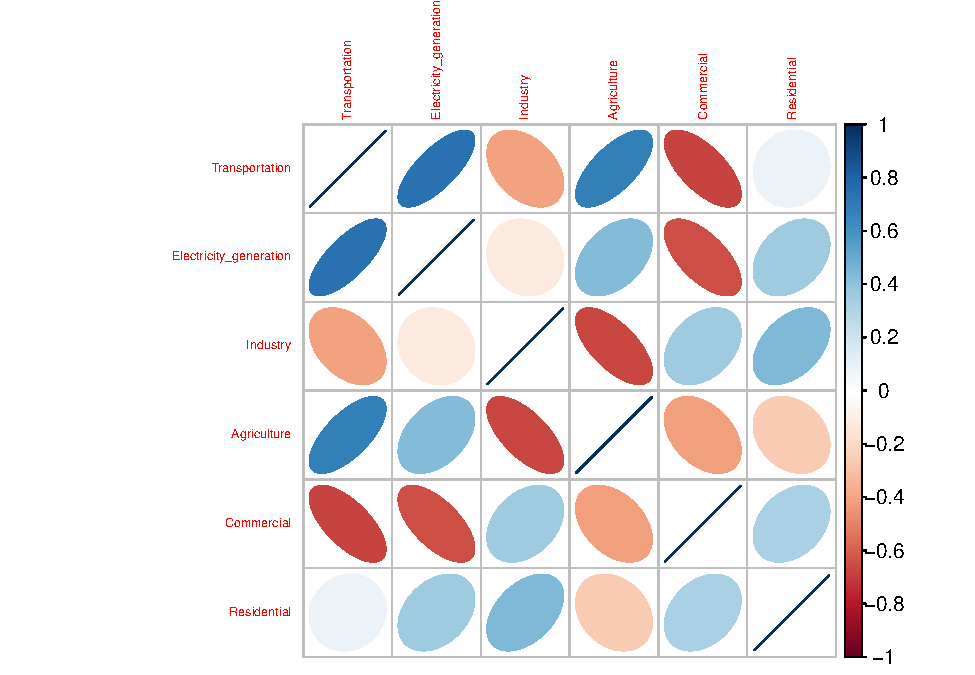
\includegraphics{Project_Code_files/figure-latex/unnamed-chunk-23-1.pdf}
\caption{Correlation Plot of US GHG Emission by Sector}
\end{figure}

\newpage

\subsubsection{Did total electricity consumption differ among
sectors?}\label{did-total-electricity-consumption-differ-among-sectors}

The first impact factor on GHG emissions to study is the domestic
electricity consumption. As illustrated in the previous section, there
was no general consumption trend among sectors. Therefore, a detailed
exploration on electricity consumption dataset was first conducted.
Specifically, this section addresses on if electricity consumptions were
significantly different among various sectors.

First, all data were gathered by sector and tested for the normality.
The normal Q-Q plot shows that the emissions were normally distributed.
Then, one-way Anova was tested, reflecting that electricity consumptions
were significantly differed among various sectors (ANOVA, R2=0.2598, dF
= 81, p \textless{} 0.0001). A post-hoc test was then run to look at the
pairwise differences, and the result was shown in Figure 9, which
illustrates that three sectors were significantly different from each
other.

\begin{figure}
\centering
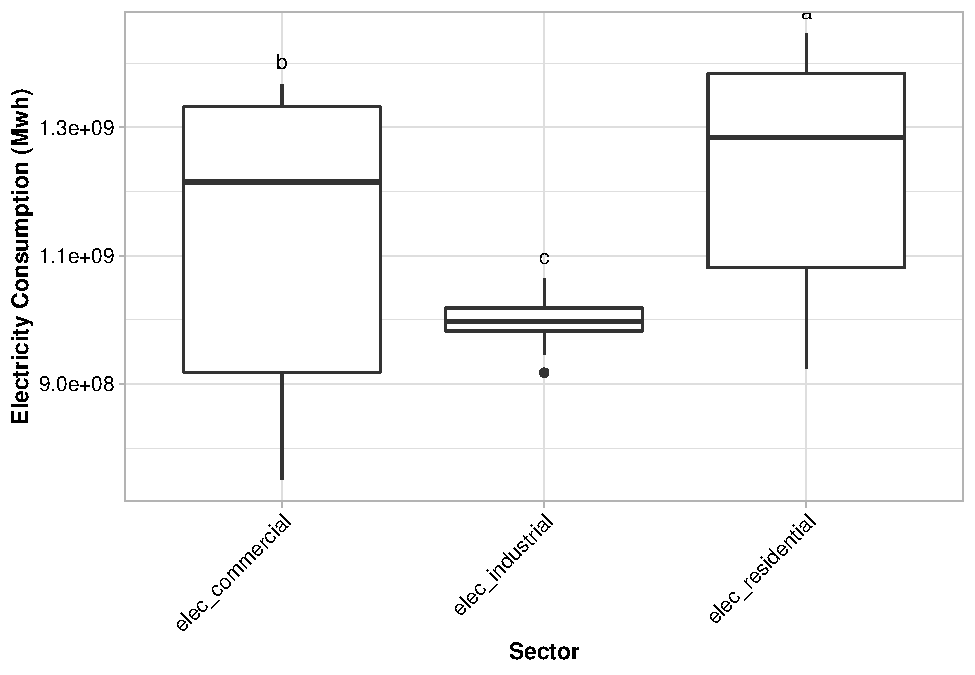
\includegraphics{Project_Code_files/figure-latex/unnamed-chunk-25-1.pdf}
\caption{Post-hoc Test Plot - Pairwise Relationship between Emissions
and Sectors}
\end{figure}

\newpage

\subsubsection{Were electricity comsupmtions significant to total GHG
emissions?}\label{were-electricity-comsupmtions-significant-to-total-ghg-emissions}

After looking at two datasets themselves, this section starts to
answering the first question mentioned in the introduction - if the
electricity consumption was significant to total GHG emissions. A
multiple linear regression was run to see the relationship. The result
showed that there was no significant relationship between electricity
consumption and total GHG concentrations (linear regression, R2=0.2623,
dF = 24, p = 0.05896), among which elec\_industrial sector was the only
significant variable. Since the p-value was close to 0.05 significane
level, the AIC test was conducted to see the better model. The improved
model was the test between the total GHG emission and electricity
consumption in industrial sector (Step: AIC=321.5), and the result from
the linear regression also indicated the significant relationship
between them (linear regression, R2=0.1774, dF = 26, p = 0.0214).

The relationships of three explanatroy data with total GHG concentration
were illustrated in Figure 10, in which commerncial electricity
consumption data and residential electricity consumption data are away
from the respective regression line, which results in the insignificant
relationships with total GHG concentration.

\begin{figure}
\centering
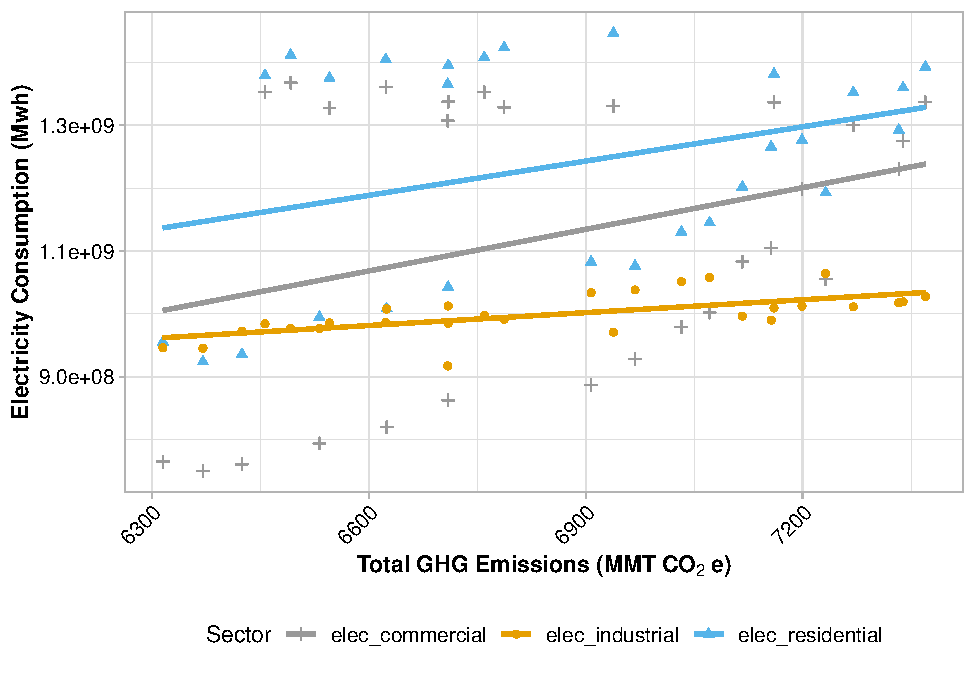
\includegraphics{Project_Code_files/figure-latex/unnamed-chunk-27-1.pdf}
\caption{Relationships between Total GHG Emissions and Electricity
Consumptions}
\end{figure}

\newpage

\subsubsection{Is population growth significant to total GHG
concentration?}\label{is-population-growth-significant-to-total-ghg-concentration}

Another factor that might affect GHG concentration attributed to human
activities is population growth. This question was inspired by observing
from the increasing trends of both GHG emissions and population. The
shapiro test showed that the population data was normally distributed (W
= 0.95398, p-value = 0.249). Then, a simple linear regression was
conducted, which illustated there was no significant relationship
between total GHG emissions and population growth (linear regression, R2
= 0.0007, dF = 26, p = 0.8948). The relationship between these two
variables was displayed in Figure 11, which is not in a linear
relationship.

\begin{figure}
\centering
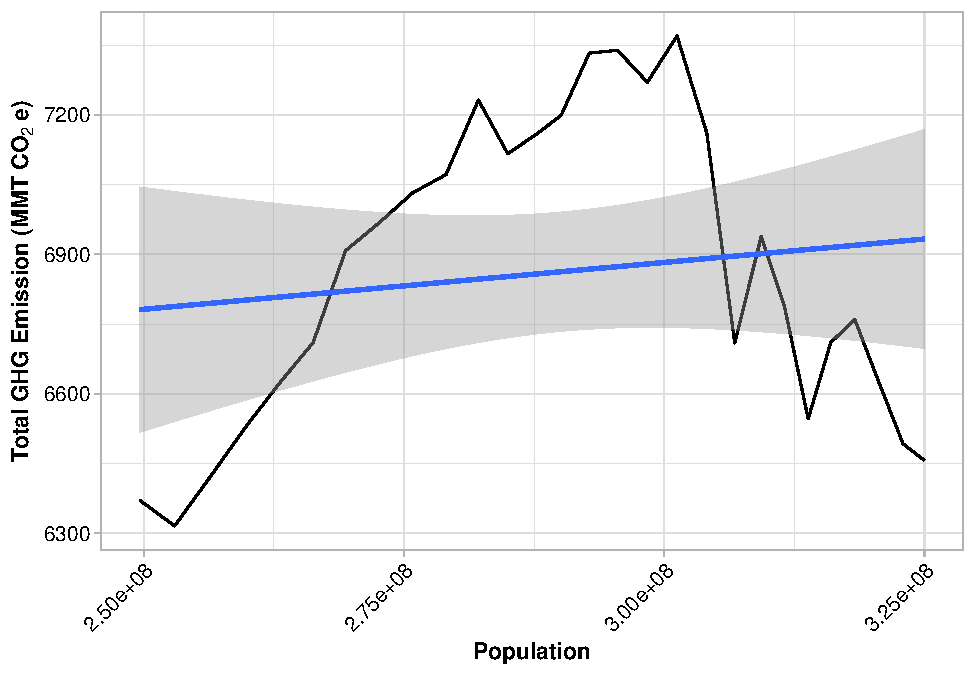
\includegraphics{Project_Code_files/figure-latex/unnamed-chunk-29-1.pdf}
\caption{Relationship between Population and Total GHG Emissions}
\end{figure}

\newpage

\subsection{Question 2: What were impacts of GHG emissions in these 28
years?}\label{question-2-what-were-impacts-of-ghg-emissions-in-these-28-years}

\subsubsection{Which sectors of GHG emissions were significant to
temperature
anomaly?}\label{which-sectors-of-ghg-emissions-were-significant-to-temperature-anomaly}

Temperature is one of the most explicit impacts of GHG emissions.
Instead of looking at sepcific types of GHGs, this project addresses on
the impacts of sectoral emissions on the temperature change, and aims to
figure out which sector was significant to the temperature.

The first step to achieve such goal was to study the chaning trend of
temperature, specifically conducting a timer series analysis to see how
the temperature had change over the 28-year period in US. The result
showed that there was no significant trend of temperature change over
the period of 1990-2017 in US (Mann-Kendall trend test z=1.758, p-value
= 0.07869).

Then, the shapiro.test was conducted to confirm the normality of
temperature anomaly data for the preparation of the linear regression (W
= 0.98866, p-value = 0.9863). The result from the multiple linear
regression illustarted that there was a significant relationship between
temperature anomaly and sectoral emissions (linear regression, R2 =
0.8219, dF = 21, p \textless{} 0.0001). Specifically, emissions from
transporation sector, agriculture sector, and residential sector were
significant to such change. An AIC test were computed to improve the
model to best illustrate explanatory variables in such a relationship,
and the improved model included transportation, agiculture, commercial,
and residential sectors (Step: AIC=-42.11). The multiple linear
regression result proved that all of these sectoral emissions were
significant to temperature anomaly (linear regression, R2 = 0.816, dF =
23, p \textless{} 0.0001).

A correlation plot was then created to visualize the correlationship and
covariance between these variables. As shown in Figure 12, residential
emissions and commercial emissions were mroe correlated to temperature
anomaly changes in negative trends, while transportation emission and
agriculture emissions were correlated to temperature anomaly in positive
trends.

\begin{figure}
\centering
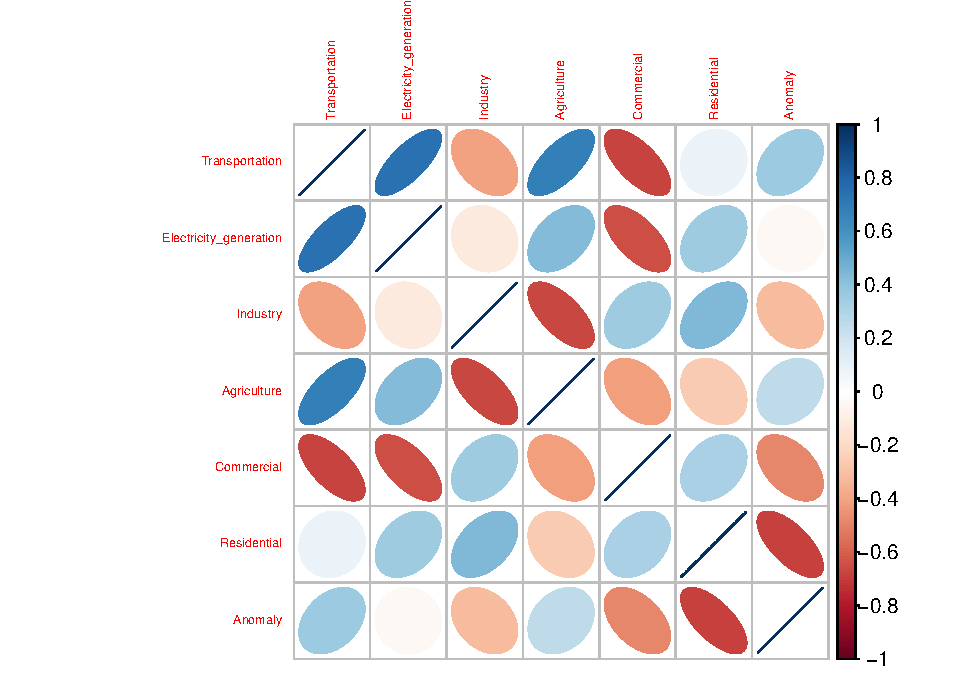
\includegraphics{Project_Code_files/figure-latex/unnamed-chunk-31-1.pdf}
\caption{Correlation Plot between US Mean Annual Temperature Anomaly and
Sectoral GHG Emissions}
\end{figure}

\subsubsection{Was total GHG emissions significant to GDP
growth?}\label{was-total-ghg-emissions-significant-to-gdp-growth}

As most GHGs were emitted by human activities, were such emissions
significant to economic development? In this proejct, GDP was selected
as the parameter to assess economic development. A similar time series
analysis was conducted to assess if GDP had change over the study period
in US. The result showed that there was a significant increasing trend
of GDP change over the period of 1990-2017 in US (Mann-Kendall trend
test z= 5.05, p-value \textless{} 0.0001).

GDP data was normally distributed according to shapio.test (W = 0.9486,
p-value = 0.1827). However, there was no significant relationship
between total GHG emissions and GDP growth over the time (linear
regression, R2 = 0.0004, dF = 26, p = 0.7499). Such result was
visualized in Figure 13, which illustrates that variables were dispersed
away from the linear trend line.

\begin{figure}
\centering
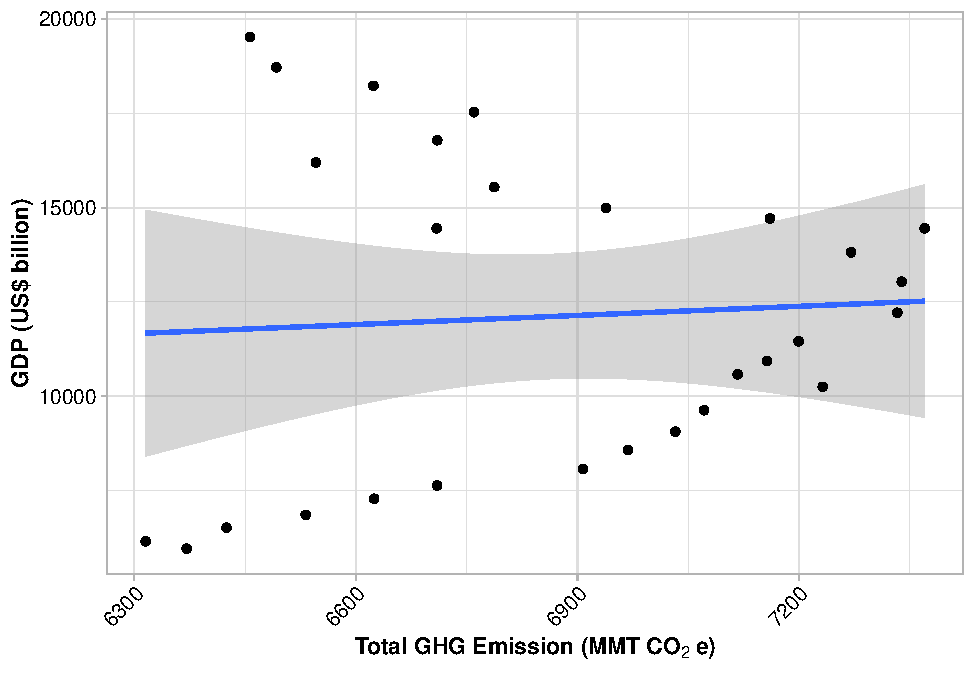
\includegraphics{Project_Code_files/figure-latex/unnamed-chunk-33-1.pdf}
\caption{Relationship between US GDP and Total GHG Emissions}
\end{figure}

\newpage

\section{Summary and Conclusions}\label{summary-and-conclusions}

As Global Warming is a more server problem, GHG emissions as one of the
most responsible factors are addressing more people's attention. This
project studies the factors that might contribute to GHG emissions and
also the potential impacts of GHG emissions in US from 1990-2017.

The first part of the project looked at the electricity consumption of
which sector is significant to total GHG emissions and examined if
population growth is significant to total GHG emission during this
period. The tests from linear regression revealed that industrial
electricity consumption was significant to total GHG emissions, and
there was no significant relationship between population growth and
total GHG emissions. In this section, the relationships among different
types of GHGs as well as the relationships among sectoral emissions were
also explored. By running different types of generalized linear models,
the results illustrated that in 1990-2017:

\begin{enumerate}
\def\labelenumi{\arabic{enumi}.}
\tightlist
\item
  CH4 and N2O emissions were significantly related to CO2 emissions;\\
\item
  CH4 and Fgas were strongly correlated;\\
\item
  Emissions in agriculture, commercial, and residential sectors were
  significantly related to emissions in electricity generation sector;\\
\item
  Electricity consumptions were significantly different among various
  sectors.
\end{enumerate}

The second part analyzed the potential impacts of GHG emissions,
specifically referring to temperature anomaly changes and GDP growth.
Time series analysis was first conducted to evaluate how these two
variables have changed over time, and the results demonstrated that
there was no significant trend of temperature, and there was a
significant increasing trend of GDP over 28 years. For temperature
change, emissions in transportation, agiculture, commercial, and
residential sectors were most significant to temperature anomalies;
however, there was no significant relationship between total GHG
emissions and GDP growth over the period.

This project is still a prelinary research on analyzing socioeconomic
factors and impacts GHG emissions with many limitations. For example,
the temporal range - 28 years - is short. Such factor was restricted by
the data availability, while the GHG emissions always have a lag
effects; that says, the impacts of GHG emissions, especially on
temperature change, will not be revealed immediately. Also, the study on
temperature change should be considered at a long-term scale, i.e.~from
pre-industrial period. Also, the geographic scale is also too broad.
Different states in US have their only regulatories on GHG emissions,
such as California as a leader on reducing GHG emissions over a long
time. The analysis at the national level cannot illustrte the progress
of policy inplementation. However, this project is still helpful to
learn from the past about the causes and consequences of GHG emissions,
as a reference as well as a warning to decision markers to think about
the environmental impacts of emissions in the future.


\end{document}
